\chapter{Introduction}
\label{ch:chapter_1}
 
\epigraph{
    “Did I mention that I know almost everything about almost everything ?”
}{Dr. Rodney McKay, fictional character}

\begin{abstract}
Molecular electronics is a relatively young field that attempts to find functional molecular junctions, initially as an alternative to semiconductor devices reaching atomic limits. In this chapter, I sketch both the experimental and theoretical context in which this thesis is placed.
\end{abstract}

%% Start the actual chapter on a new page.
\newpage
\section{Molecular Electronics}
Modern electronics is almost entirely based on semiconductor physics. The most abundant and thus primary element for electronics is silicon. Since the 1960, efforts have been made to minimise the semiconductor devices to ever smaller scales. However, semiconductors are bulk materials, implying a fundamental limit to their minimisation. Now that the downsizing approaches molecular scales, it is at its end ~\cite{seldenthuis}.

The next smallest functional element is a molecule. Evolution by natural selection has, at the biochemical scale, led to a very broad spectrum of functional molecules. A great amount of molecules can be synthesised by utilising the specialised enzymes provided in that way.

At the molecular scale, new functionality also arises. For instance, molecules can respond to light and heat. They can act as logic gates, rectifiers, solar cells and much more ~\cite{perrin}. Experts see the most exciting future of the field in that direction, in new functional elements rather than replacement of semiconductor elements ~\cite{visions}.

Fundamental to the creation of molecular devices is the understanding of their fabrication and behaviour . My thesis focuses almost entirely on the latter aspect, although previous experiments will be discussed as a way of confirming or motivating theoretical work.

It is useful to be aware of some experimental issues. For instance, the contacting of a single-molecule in a device is non-reproducible . Statistical approaches to measure conductance and other molecular properties are essential. The challenge lies partially in reducing the variability or to exploit molecular functionalities that are insensitive to the details of the contacts ~\cite{visions}.

For theory, on the other hand, the challenge lies in removing the mismatch between theory and experiment. In particular, predicting transport gaps and determining location of (frontier) orbital levels with respect to the Fermi energy have proven very challenging~\cite{perrin}. Primarily I focus on incorporating interactions into the formalism. Normally, only single-electron transport is considered, partially because the appropriate formalism  was not available. Starting from a note by Dr. Jos Seldenthuis, I develop the appropriate formalism. I apply this to a model, thereby incorporating Coulomb interactions, that has been shown to qualitatively work well to explain the behaviour of thiolated arelythynylene with a dihydroanthracene core ~\cite{perrinnano}. I also consider a similar model that incorporates spin, although its novelty originates in that it is now imperative to consider it because of interactive effects where it was originally a trivial spin-splitting. 
%%%%%%%%%%%%%%%%%%%%%%%%%%%%%%%%%%%%%%%%%%%%%%%%%%%%%%%%%%%%%%%%%%%%%%%%%%%%%%%%%%%%%%%%%%%%%%%%%%%%%%%%%%%%%%%%%%%%%%%%%%%%%%%%%
\section{Experimental}
I will shortly review a number of the more popular techniques for single-molecule experiments. To wit, these are Conductive Atomic Force Microscopy (C-AFM), Scanneling Tunneling Microscopy (STM), Electromigration and finally Mechanically Controlled Break Junctions (MCBJ). I think it important to have some knowledge of the experimental reality of the nanoscopic devices I investigate theoretically.

Atomic Force Microscopy is a type of scanning probe microscopy with resolution of less than a single nanometre. By using a piezoelectric element, it can make an accurate surface scan by keeping the forces between probe and sample constant~\cite{frei1, frei2}.

For molecular electronics, molecules are evaporated onto the gold substrate. The AFM tip, a golden cantilever, is brought into contact with a substrate and slowly retracted. The evaporated molecules form a self-assembled mono layer, so that some molecules have migrated onto the substrate-tip bond. As it breaks, a molecular break junction is formed. However, this requires conductive molecules, which is why the technique is referred to as Conductive-AFM (C-AFM). Also, it is relevant that usually C-AFM measurements concern groups of molecules, only rarely a single molecule.

The AFM method has several features. First, it can measure both electrical current and forces in a parallel measurement~\cite{nef}. Another large advantage is that the topographic imaging and electrical measurement are simultaneously achieved, so that the nano-device is relatively well documented before measurement ensues.

The Scanneling Tunneling Microscopy method features similar advantages ~\cite{Joachim2000}, but instead of using a golden cantilever it is the scanning probe tip that is brought into contact with a molecule, and then very slowly pulled away. The molecule, which bonds to the tip, is the stretched between the substrate and the STM tip, making another (gold) molecular junction.

Electromigration is a method of gap formation that makes use of increased mobility due to the application of voltage. An overlapping set of gold leads is made, which is subject to voltage ramps at ambient laboratory conditions. The voltages increase the mobility of the gold atoms, which move away from the future gap. The gap formed by this method is highly irreproducible~\cite{electromigration}.

Finally, the Molecular Controlled Break Junction is the technique used by~\citet{perrinnano}, whose work I will discuss later in section~\ref{sec:perrin}. In figure~\ref{fig:mcbj} the basic setup of a Mechanically Controllable Break Junction (MCBJ) is shown~\citet{perrin} . These offer high electrode stability and fine-tuning of the electrode spacing. 
\begin{figure}[!bp]
    \centering
    \includegraphics[height=0.3\textheight,page=2, clip=true, trim=2.5cm 16.5cm 11cm 6cm]{pdf/perrinnnano.pdf}
    \caption{Schematic drawing of a MCBJ. A Gold wire is deposited on top of a flexible substrate, which is then bend by the three-point mechanism. The wire breaks, forming a size-controllable gap.}
    \label{fig:mcbj}
\end{figure}

The working principle behind the MCBJ technique is to deposit a thin metallic wire on top of a flexible substrate. Gold is often used because it is a noble metal. By bending the substrate in a three-point mechanism, the gold wire stretches and breaks. It then forms two gold surfaces, the electrodes. The spacing between these electrodes can be tuned by adjusting the bending of the sample. The junction can be reformed after it is broken.

The allowed voltage over such a MCBJ junction ranges from $0.5$ V at room temperature up to $2$-$3$ V at $4.2$K. At low temperatures, the size of the gap does not significantly change over time. Additionally, the technique allows repeated fusing and breaking, and is thus ideal for statistical studies which are required for mechanistic insight because of the large fluctuations in experiments ~\cite{ratnerrev2013}.

A few examples of experimental findings~\cite{koole} involving molecular electronics are the Coulomb blockade~\cite{Park2000, Park2002}, the Kondo effect~\cite{Park2002}, vibrational excitations~\cite{vib1, vib2} and electronic excitations~\cite{elec1}.

\section{Theory}
\label{sec:theoryintro}
While I work primarily in the non-equilibrium Green's Function Formalism (chapter~\ref{ch:chapter_2}), here I will also briefly describe another formalism often used, namely the Master Equation approach ~\cite{seldenthuis}. One very large benefit of the Master Equation approach over the non-equilibrium Green's Function approach is that it has a simple conceptual interpretation.

Let us start by noting that molecules can be viewed as a collection of quantum dots. For instance, consider a simple chain of carbon atoms, with transport dominated by a single atomic orbital. It makes sense that one can describe this chain with the simplified model of a chain of quantum dots with a single energy level for each individual dot, thereby leading to 4 orbital levels of the molecule. If spin is included, the system could even be described as a chain of Qubits.

The typical way of physicist thinking is the Master Equation (ME) approach. The ME approach is only valid for weak coupling, so it is technically not relevant for a chain of carbon atoms. However, the chain of carbon atoms was only a parable with the aim of establishing the collection of quantum dots picture.

If one considers one of these dots centred between two others ($c$) , then one needs to know the rate $W$ at which electrons leave it to either the right ($r$ or the left ($l$) neighbouring dot, and the rate at which they enter. Of course, the net flux depends on the chances $P$ the neighbouring dots are occupied. For instance, the flux of electrons coming from the left is the chance that the left dot is occupied $P_l$ times the rate $W_{l\rightarrow c}$ of electrons moving from the left ot the central dot. Based on this simple reasoning, I formulate the Master Equation ~\cite{beenakker}:
\begin{align*}
\frac{d}{dt} P_c &= P_l W_{l\rightarrow c} - P_c W_{c\rightarrow l} + P_r  W_{r\rightarrow c} - P_c W_{c\rightarrow r}.
\end{align*}

Of course, I have not yet specified the rates of leaving and entering the central dot. However, note that the master equation is linear and can be written in matrix form, $\dot{P} = W P$. For a more elaborate system, the system would have multiple states on each dot, and fluxes would look like e.g. $P_{li} W_{li\rightarrow cj}$, denoting the flux of electrons that occupied the left dot in a numbered state $i$ to the central dot in state $j$.  

Any molecule has as its constituents the atoms and the electrons. Generally the atomic background of the electrons is approximated as an effective potential. However, it is known that molecules can have nuclear motion, which can feature in transport as well, e.g. phonon interactions also known as vibrational modes. I therefore use the Born-Oppenheimer approach (section~\ref{sec:schrodinger}), where it is assumed the wave-function $\ket{\Psi}$ is separable into the atomic nuclei state $\ket{\phi}$ and the electronic state $\ket{\psi}$. The rates due to a (weak) interaction $H'$ be found from the well-known Fermi's Golden rule between initial state $\ket{i}$ and final state $\ket{f}$:
\begin{align*}
W_{i\rightarrow f}  &= \frac{2\pi}{\hbar} \left| \braket{\Psi_f \left|H'\right| \Psi_i}\right|^2 \rho_f (\epsilon_f)  \\
&= \frac{2\pi}{\hbar} \left| \braket{\phi_f \psi_f \left|H'\right| \phi_i \psi_i}\right|^2 \rho_f (\epsilon_f),
\end{align*}
where $\rho_f(\epsilon_f)$ denotes the final density of states. 

The atomic overlap $\left| \braket{ \phi_f | \phi_i }\right|^2$ is known as a Franck-Condon factor (section~\ref{sec:phononic}). Note that different electronic eigenstates very often have a slightly different atomic state, implying that the Franck\hyp{}Condon factor between non-identical states become non-zero. Theoretically, this can be understood as a basis change; $\ket{\phi_i}$ and $\ket{\phi_f}$ are no longer pure eigenstates in the new basis. 

The ME approach is very suited to handling vibrational excitations and interactions up to any desired order ~\cite{seldenthuis}. One particular feature of the ME approach is that the ME approach assumes that electrons remain on a `dot' for long times, losing all phase information. Therefore, quantum interference is a feature that the ME approach does not cover, thereby requiring that the level spacing is larger than the effective coupling $\delta \epsilon_i \gg \Gamma$. The non-equilibrium Green's Function Formalism (chapter~\ref{ch:chapter_2})  does not lose phase information and can thus calculate quantum interference. Additionally, the ME approach covers weak coupling while the NEGF formalism covers strong coupling.

Both the ME approach and the NEGF formalism deal with molecules; small functional blocks. However, you need to characterise the molecule or at the very least its single-electron orbitals at the HOMO and LUMO level. 

I will now describe Density Functional Theory (DFT) as it pertains to transport calculations for single-molecule junctions. This theory is very well known and recognised, as demonstrated by the 1998 Nobel Prize in Chemistry, shared equally between Walter Kohn "for his development of the density-functional theory" and John A. Pople "for his development of computational methods in quantum chemistry"~\cite{nobel1998}. 

The starting point of DFT is that the ground-state density $n(r^\mu)$ for any (possibly interacting) electronic system uniquely determines the system. Effective approxim\-ations for the functionals involved in DFT lead to the DFT calculations of today (e.g. LDA, GGA). 

Let us describe, briefly, the general approach of DFT. DFT starts with some initial guess $n^0(r^\mu)$ \footnote{I denote the positions of atoms as $r^\mu = (x,y,z)$.}. Using this guess, in practise the DFT approach constructs a Schr\"odinger equation which depends on the electron density rather than the individual electron orbit\-als~\cite{joscomp}. Solving this Schr\"odinger equation leads to a new density, $n^1(r^\mu)$, which is then used to construct a new Schr\"odinger equation. This iterative self-consistency loop is broken when the electron density converges.

As a specific DFT example, the Kohn-Sham approach minimises the single-particle Kohn-Sham equations ~\cite{kohnsham, joscomp}:
\begin{align}
\left( -\frac{1}{2} \nabla^2 + v_\text{eff} (r^\mu) - \epsilon_i \right) \varphi_j( r^\mu) &= 0, \label{eq:ks}
\end{align}
with
\begin{align*}
n(r^\mu) &= \sum_{j=1}^N \left| \varphi_j (r^\mu)\right|^2,\\
v_\text{eff} &= v(r) + \int \frac{n(x^\mu)}{\left|r^\mu - x^\mu\right|} dx^\mu + v_\text{xc}(r^\mu),
\end{align*}
where $v_\text{xc}(r^\mu)$ is the local exchange-correlation potential, a chosen functional that depends on the density distribution $n(r^\mu)$ of the current iteration. The external potential $v(r)$ which, in the systems of interest, is the Coulomb attraction by the static nuclei.


I have now described the basic process of a DFT calculation. Depending on the implementation, a basis set might have to be chosen in addition to the exchange\hyp{}correlation functional.The DFT calculation returns the Hamiltonian of the system formulated in the chosen basis. To this Hamiltonian the non-equilibrium Green's Function Formalism (chapter~\ref{ch:chapter_2})can be applied, although it exists independently for a non-equilibrium system, such as a molecule coupled to one or more electron bath(s). I will discuss this formalism at length for both arbitrary and model Hamiltonians.

\section{Outline of thesis}
In this M.Sc. Thesis, the focus lies on interactions in the non-equilibrium Green's function formalism, specifically capacitive interactions. The Coulomb interaction is capacitive and it can be incorporated into the NEGF formalism.

First, in chapter~\ref{ch:chapter_2} I derive the non-equilibrium Green's Function formalism from first principles for a generic Hamiltonian $H$. Next, I consider the derivation that incorporates interactions in chapter~\ref{ch:chapter_3}. The first and most important result of this thesis are the capacitive interactions of section~\ref{sec:capacitive}, but I will also took a brief look at vibrational excitations.

I then apply the new theory  in chapter~\ref{ch:chapter_4}. Specifically, I apply it on the two site model Hamiltonian used in ~\citet{perrinnano} and discuss the results. Finally, in chapter~\ref{ch:chapter_5} I discuss the findings and implications of the new theory. I also summarise the thesis and make suggestions for future research.

%clearpage dumps all images in the stack. Also prevents images from skipping chapters.
\clearpage
\references{dissertation}